% Niveau :      PCSI *
% Discipline :  Chimie Orgam
% Mots clés :   Ballistique, Mécanique du point, PFD, Chute libre

\begin{exercise}{Synthèse de Bouveault}{2}{PCSI}
{Chimie organique I, AN,  organométallique}{bermu}
\index{AN+E}\index{amide}

\begin{questions}
\questioncours Réactivité et intérêt synthétique des organomagnésiens mixtes.

\begin{EnvUplevel}
Parmi les autres intérêts sythétiques des organomagnésiens, le chimiste français Louis Bouveault a trouvé en 1904 une voie de synthèse originale utilisant les organomagnésiens.

Partant du chlorure d'éthyle \textbf{A},
\begin{center}
    \schemestart
        \textbf{A}
        \arrow{->[Mg$^0$][DMF, reflux]}[,2.1]
        \textbf{B}
        \arrow{->[DMF][reflux]}[,1.5]
        \textbf{C}
        \arrow{->[H$^+$][H$_2$O, $0^\circ$C]}[,1.9]
        \textbf{D}
        %\chemname{\chemfig{C_3H_6O}}{\textbf{D}}
    \schemestop\chemnameinit{}~,
    \end{center}
on forme le composé \textbf{D}. DMF désigne ici le N,N-diméthylformamide : \chemfig{H-[1,.7](=[3,.7]O)-[-1,.7]N(-[-3,.7])-[1,.7]}\,.
\end{EnvUplevel}

\question Donner la structure et préciser le protocole expérimental de formation de \textbf{B}.

\question Donner la structure de l'intermédiaire \textbf{C} et le mécanisme de sa formation.

\begin{EnvUplevel}
L'espèce \textbf{C} est ensuite hydrolysée à basse température. Après lavage et séchage, l'espèce \textbf{D} est caractérisée par spectroscopie infrarouge. On donne ci-dessous les spectres des produits et des réactifs de la synthèse. \vspace{-1em}
\begin{figure}[H]
    \centering
    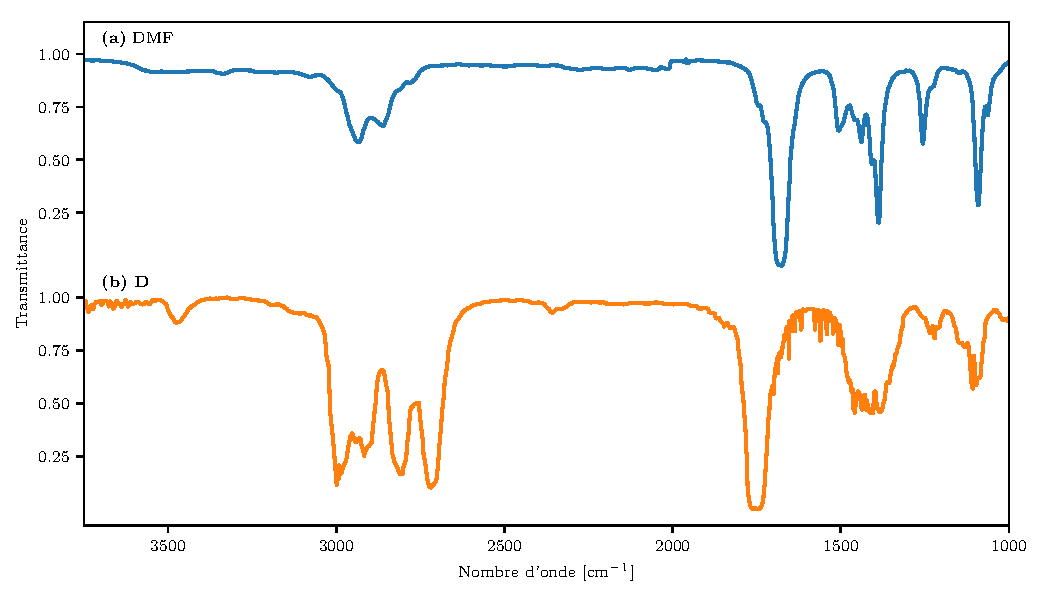
\includegraphics[width=\linewidth]{chimiePC/orga/bouveault.pdf}\vspace{-.5em}
    \caption{Spectres infrarouges du DMF \textbf{(a)} et du produit final obtenu \textbf{D (b)}.}
\end{figure}
\end{EnvUplevel}

\question Justifier les conditions expérimentales de la dernière étape.

\question Identifier sur les spectres IR ci-dessus les fonctions créées et détruites lors de la synthèse. \\
Vous pouvez vous aider si besoin d'une table IR.

\question Donner la structure de \textbf{D} et justifier le caractère nucléofuge du groupe partant lors de \textbf{C} $\longrightarrow$ \textbf{D}.

\question Proposer succinctement un protocole pour isoler \textbf{D}.

\question Proposer d'éventuels sous-produits de ce protocole expérimental.

\question Quel est l'intérêt de cette synthèse ?


\end{questions}
\end{exercise}

\begin{solution}
\begin{questions}
    \questioncours R--Mg--X est un excellent nucléophile, une excellente base (au sens de Lewis et de Brönsted) et un bon réducteur.
    
    Le carbone de R--Mg--X est chargé $\delta^-$, ce qui est très utile en chimie organique pour assembler différents édifices carbonés : moyen de créer des liasons C--C.
    
    Permet aussi de former des alcools par réaction sur les carbonylés.
    
    \question \textbf{B} : $\mathrm{CH_3}$--Mg--Br, cf{.} cours pour le protocole.
    
    \question\hfill
    \schemestart
        \chemname{\chemfig{CH_3-[@{a1},1.5,,,red]MgBr}}{\textbf{B}}
        \+
        \chemname{\chemfig{H-[1]@{b1}(=[@{a2}3]@{b2}\lewis{13,O})-[-1]\lewis{2,N}(-[-3])-[1]}}{DMF}
        \chemmove[red,-stealth,red,shorten >=3pt]{
            \draw(a1)..controls +(up:10mm) and +(north west:10mm).. (b1);}
        \chemmove[red,-stealth,red,shorten <=2pt]{
            \draw(a2)..controls +(west:2mm) and +(south west:5mm).. (b2);}
        \arrow{->}
        \chemname{\chemfig{H-[1](-[4])(-[2]O^\ominus,\:MgBr^\oplus)-[-1]\lewis{2,N}(-[-3])-[1]}}{\textbf{C}}
    \schemestop\chemnameinit{}\hfill~
    
    \question Lors de \textbf{C} $\longrightarrow$ \textbf{D}, l'eau sert à hydrolyser \textbf{C} mais aussi à détruire l'excédent de \textbf{B} et de magnésium. La réaction est très exothermique ($\Delta$pK$_a \simeq$ 20), et donc il faut la faire à basse température par précaution.
    
    \question \`A la fin de cette étape, il y a une phase organique chargée en \textbf{D} avec quelques polluants ioniques et une phase aqueuse chargée de sous-produits.
    
    On peut laver et décanter la phase organique puis évaporer le gros du solvant à l'évaporateur rotatif. Enfin, on peut isoler \textbf{D} par distillation fractionnée.
    
    \question Il n'y a pas de bande large O--H à 3500 cm$^{-1}$ comme on s'y attendrait : on ne forme donc pas un alcool. La bande C$=$O à 1700 cm$^{-1}$ se décale suggérant que l'on passe d'une amide à un carbonyle (cétone ou aldéhyde). Le pic C--N à 1150 cm$^{-1}$ disparaît.
     
    \question Penser à l'analogie entre les esters et les amides. Suggestion de mécanisme concerté (on peut l'envisager aussi en plusieurs étapes) :
    \begin{center}\schemestart
        \chemname{\chemfig{H-[1](-[4])(-[2]O^\ominus,\:MgBr^\oplus)-[-1]\lewis{2,N}(-[-3])-[1]}}{\textbf{C}}
        \arrow{->[H$^+$][$-$ MgBr$^\oplus$]}[,1.9]
        \chemname{\chemfig{H-[1](-[4])(-[@{b1}2]\lewis{23,O}-[@{a1},,,,red]@{b2}H)-[@{a2}-1,,,,red]\lewis{2,N}(-[-3])-[1]}}{\textbf{C'}}
        \chemmove[red,-stealth,red,shorten >=3pt]{
            \draw(a1)..controls +(south:5mm) and +(south east:3mm).. (b1);
            \draw(a2)..controls +(north east:4mm) and +(down:7mm).. (b2);}
        \arrow{->[][$-$ HN(CH$_3$)$_2$]}[,2.1]
        \chemname{\chemfig{-[1](=[3]O)-[-1]H}}{\textbf{D}}
    \schemestop\chemnameinit{}
    \end{center}
    
    L'amine HN(CH$_3$)$_2$ est un très bon nucléofuge car elle est une base de Lewis encombrée.
    
    \question L'amine HN(CH$_3$)$_2$ est rejetée à la suite de la seconde étape, on peut la faire passer en solution en diminuant le pH : $\mathrm{HN(CH_3)_2 + H^+ \longrightarrow H_2N^+(CH_3)_2}$. On pourrait également envisager la présence comme sous-produit de \textbf{C'}, intermédiaire pour lequel il n'y a pas eu de départ nucléofuge.
    
    \question Cette synthèse permet donc de synthétiser des aldéhydes avec des organomagnésiens ce qui est normalement compliqué car les aldéhydes sont attaqués par les organomagnésiens.
    
\end{questions}
\end{solution}